\NeedRoom{10}

\subsection{Financial and Carbon Results}

\begin{longtable}{@{}L{\dimexpr 0.16000\textwidth-2\tabcolsep\relax}L{\dimexpr 0.20000\textwidth-2\tabcolsep\relax}L{\dimexpr 0.22000\textwidth-2\tabcolsep\relax}L{\dimexpr 0.23000\textwidth-2\tabcolsep\relax}L{\dimexpr 0.19000\textwidth-2\tabcolsep\relax}@{}}
\caption{Immediate-replacement financial outcomes by grant share}\label{tab:source10}\\
\toprule
\textbf{Grant share} & \textbf{Grant (CAD m)} & \textbf{Agency PV (CAD bn)} & \textbf{NPV savings (CAD m)} & \textbf{Payback year} \\
\midrule
\endfirsthead
\multicolumn{5}{l}{Table \thetable\ (continued)}\\
\toprule
\textbf{Grant share} & \textbf{Grant (CAD m)} & \textbf{Agency PV (CAD bn)} & \textbf{NPV savings (CAD m)} & \textbf{Payback year} \\
\midrule
\endhead
\midrule\multicolumn{5}{r}{Continued on next page}\\\endfoot
\bottomrule\endlastfoot
0\% & 0.0 & 2.065 & -80.3 & 10 \\
25\% & 240.1 & 1.825 & 159.8 & 10 \\
50\% & 480.1 & 1.585 & 399.9 & 6 \\
\end{longtable}

Gross electric present cost is CAD 2.065 billion, versus CAD 1.985 billion for diesel. Break-even support is 8.4\% of the eligible initial increment. The 50\% cap is sufficient in this scenario: true. These are conditional screens, not contract forecasts.


\begin{figure}[htbp]\centering

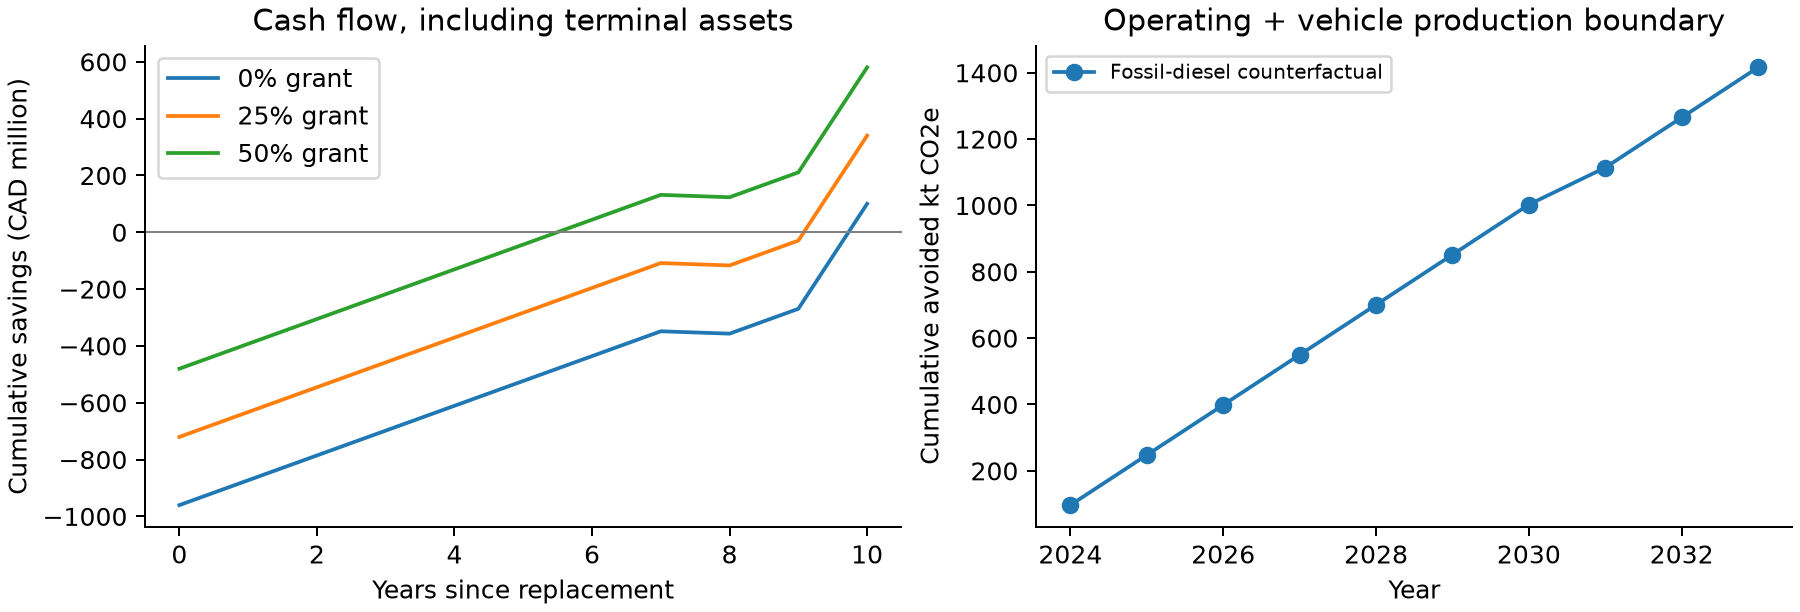
\includegraphics[width=\textwidth,height=0.37\textheight,keepaspectratio]{images/environment_finance.png}

\caption{Cumulative cash savings, with terminal credits in the final year, and emissions avoided within the stated boundary.}\label{fig:result2}

\end{figure}

Gross discounted TCO is CAD 2.22 per electric vehicle-km and CAD 2.40 per diesel vehicle-km. Own-mileage denominators differ because deadhead differs; the service obligations remain the same.

